%%% Andrea Quezada
%%% andreagtzq@gmail.com
%%% Twitter: @andreaquezadaa

%%% About: nice template for a cv
%%% Features: 
%%%% 1) Month is updated automatically; 
%%%% 2) It uses fontspec, some compilers do not support it
%%%% 3) Bibliography is divided in several parts: Peer-review Articles, Articles under review, Book Chapters, Proceedings and "In preparation articles". Each of them must have their .bib file.  In some compilers you will need to run the following command on the terminal for each .bib file: "bibtex file.aux"   after compile the document and then compile again. This will generate .bbl files.
%%%% 4) Including a photo is optional

%-----------------------------------------------------------
\documentclass[letterpaper,11pt]{article}
\renewcommand{\familydefault}{\rmdefault} 
\newlength{\outerbordwidth}
\pagestyle{empty}
\raggedbottom
\raggedright
\usepackage[english]{babel}
\usepackage[utf8]{inputenc}                 
\usepackage{ragged2e}
\usepackage{graphicx}
\usepackage[scale=0.75]{geometry}
\usepackage[svgnames]{xcolor}
\usepackage{framed}
\usepackage{tocloft}
\usepackage{ragged2e}
\usepackage{titlesec}
\usepackage{multicol}
% links
\usepackage{hyperref}
% font awesome
\usepackage{fontspec}
\usepackage{fontawesome}
\usepackage{academicons}
\definecolor{orcidlogocol}{HTML}{A6CE39}
% page numbering
\pagenumbering{arabic}
% Define colors for sections and subsections
% Find more colors at https://latexcolor.com/
\definecolor{ceruleanblue}{rgb}{0.16, 0.32, 0.75}
\definecolor{carolinablue}{rgb}{0.6, 0.73, 0.89}
\titleformat{\subsection}
{\Large\bfseries}
{\titlerule\vspace{1pc}\thesection\color{carolinablue}}
{1em}
{}
[{\color{carolinablue}\titlerule[0.8pt]}] 
%%%%% The following commands set up the Bibliography in several parts: Peer-review Articles, Articles under review, Book Chapters, Proceedings and "In preparation articles". Each of them must have their .bib file. They also rename the headings according and take out the numbers using textbullets instead. 
\usepackage{multibib}
\newcites{articles,underreview,bookchaps,proceedings,preparation}{{\normalsize{JCR-indexed Journal Articles}}, \normalsize{Publications under review}, \normalsize{Book Chapters},\normalsize{Conference Proceedings}, \normalsize{Publications in preparation}} 
\providecommand\BibTeX{{B\kern-.05em{\sc i\kern-.025em b}\kern-.08em \TeX}}
\makeatletter
%\renewcommand\@biblabel[1]{\textbullet}
\makeatother
%-----------------------------------------------------------
%Margin setup
\setlength{\evensidemargin}{-0.25in}
\setlength{\headheight}{0in}
\setlength{\headsep}{0in} 
\setlength{\oddsidemargin}{-0.25in}
\setlength{\paperheight}{11in}
\setlength{\paperwidth}{8.5in}
\setlength{\tabcolsep}{0in}
\setlength{\textheight}{9.5in}
\setlength{\textwidth}{7in}
\setlength{\topmargin}{-0.3in}
\setlength{\topskip}{0in}
\setlength{\voffset}{0.1in}
%-----------------------------------------------------------
% Use the current date every time you compile
\newcommand{\todaydo}{\ifcase \month \or January\or February\or March\or %
April\or May \or June\or July\or August\or September\or October\or November\or %
December\fi, \number \year}
%-----------------------------------------------------------
\begin{document}

% Personal Data without photo
% 
% \begin{tabular*}{7in}{l@{\extracolsep{\fill}}r}
% \textbf{\LARGE Andrea Quezada, PhD.} & \vspace*{0.2cm}\\
% \textbf{\large{Curriculum Vit\ae}} &  \\
% Last update: \textbf{\todaydo} &   \\
%\textcolor{orcidlogocol}{\faWhatsapp} (+52) 55 44 88 44 32 & \textcolor{ceruleanblue}{\faLinkedinSquare} \href{https://www.linkedin.com/in/andrea-quezada-8b64353a/}{Andrea Quezada}  \\
%  \textcolor{ceruleanblue}{\faEnvelope}  \href{mailto:agquezada@fc.ul.pt}{agquezada@fc.ul.pt}  & 
% \textcolor{orcidlogocol}{\aiOrcid} \href{https://orcid.org/0000-0002-5805-893X}{0000-0002-5805-893X} \\
% {\faEnvelopeO}  \href{mailto:andreagtzq@gmail.com}{andreagtzq@gmail.com} & {\faGithub} \href{https://github.com/andreaquezada}{andreaquezada} \\  
% \end{tabular*} 
%-----------------------------------------------------------
% Personal Data with photo
%
\begin{tabular*}{7in}{l@{\extracolsep{\fill}}r}
\begin{minipage}[h]{0.5\textwidth}\textbf{\LARGE Andrea Quezada, PhD.} \vspace*{0.2cm}
\\  \textbf{\large{Curriculum Vitae}} \\ Last update: \textbf{\todaydo}
 \\ \textcolor{ceruleanblue}{\faLinkedinSquare} \href{https://www.linkedin.com/in/andrea-quezada-8b64353a/}{Andrea Quezada}
 \\ \textcolor{ceruleanblue}{\faEnvelope}  \href{mailto:agquezada@fc.ul.pt} {agquezada@fc.ul.pt}  \\
 {\faEnvelopeO}  \href{mailto:andreagtzq@gmail.com}{andreagtzq@gmail.com}
\\\textcolor{orcidlogocol}{\aiOrcid} \href{https://orcid.org/0000-0002-5805-893X}{ORCID:0000-0002-5805-893X}  \\  
 {\faGithub} \href{https://github.com/andreaquezada}{andreaquezada} \\
 \textcolor{orcidlogocol}{\faWhatsapp}{(+351) 913 821 672} \\
  \end{minipage}
& \hspace{3cm} \begin{minipage}[h]{1\textwidth}  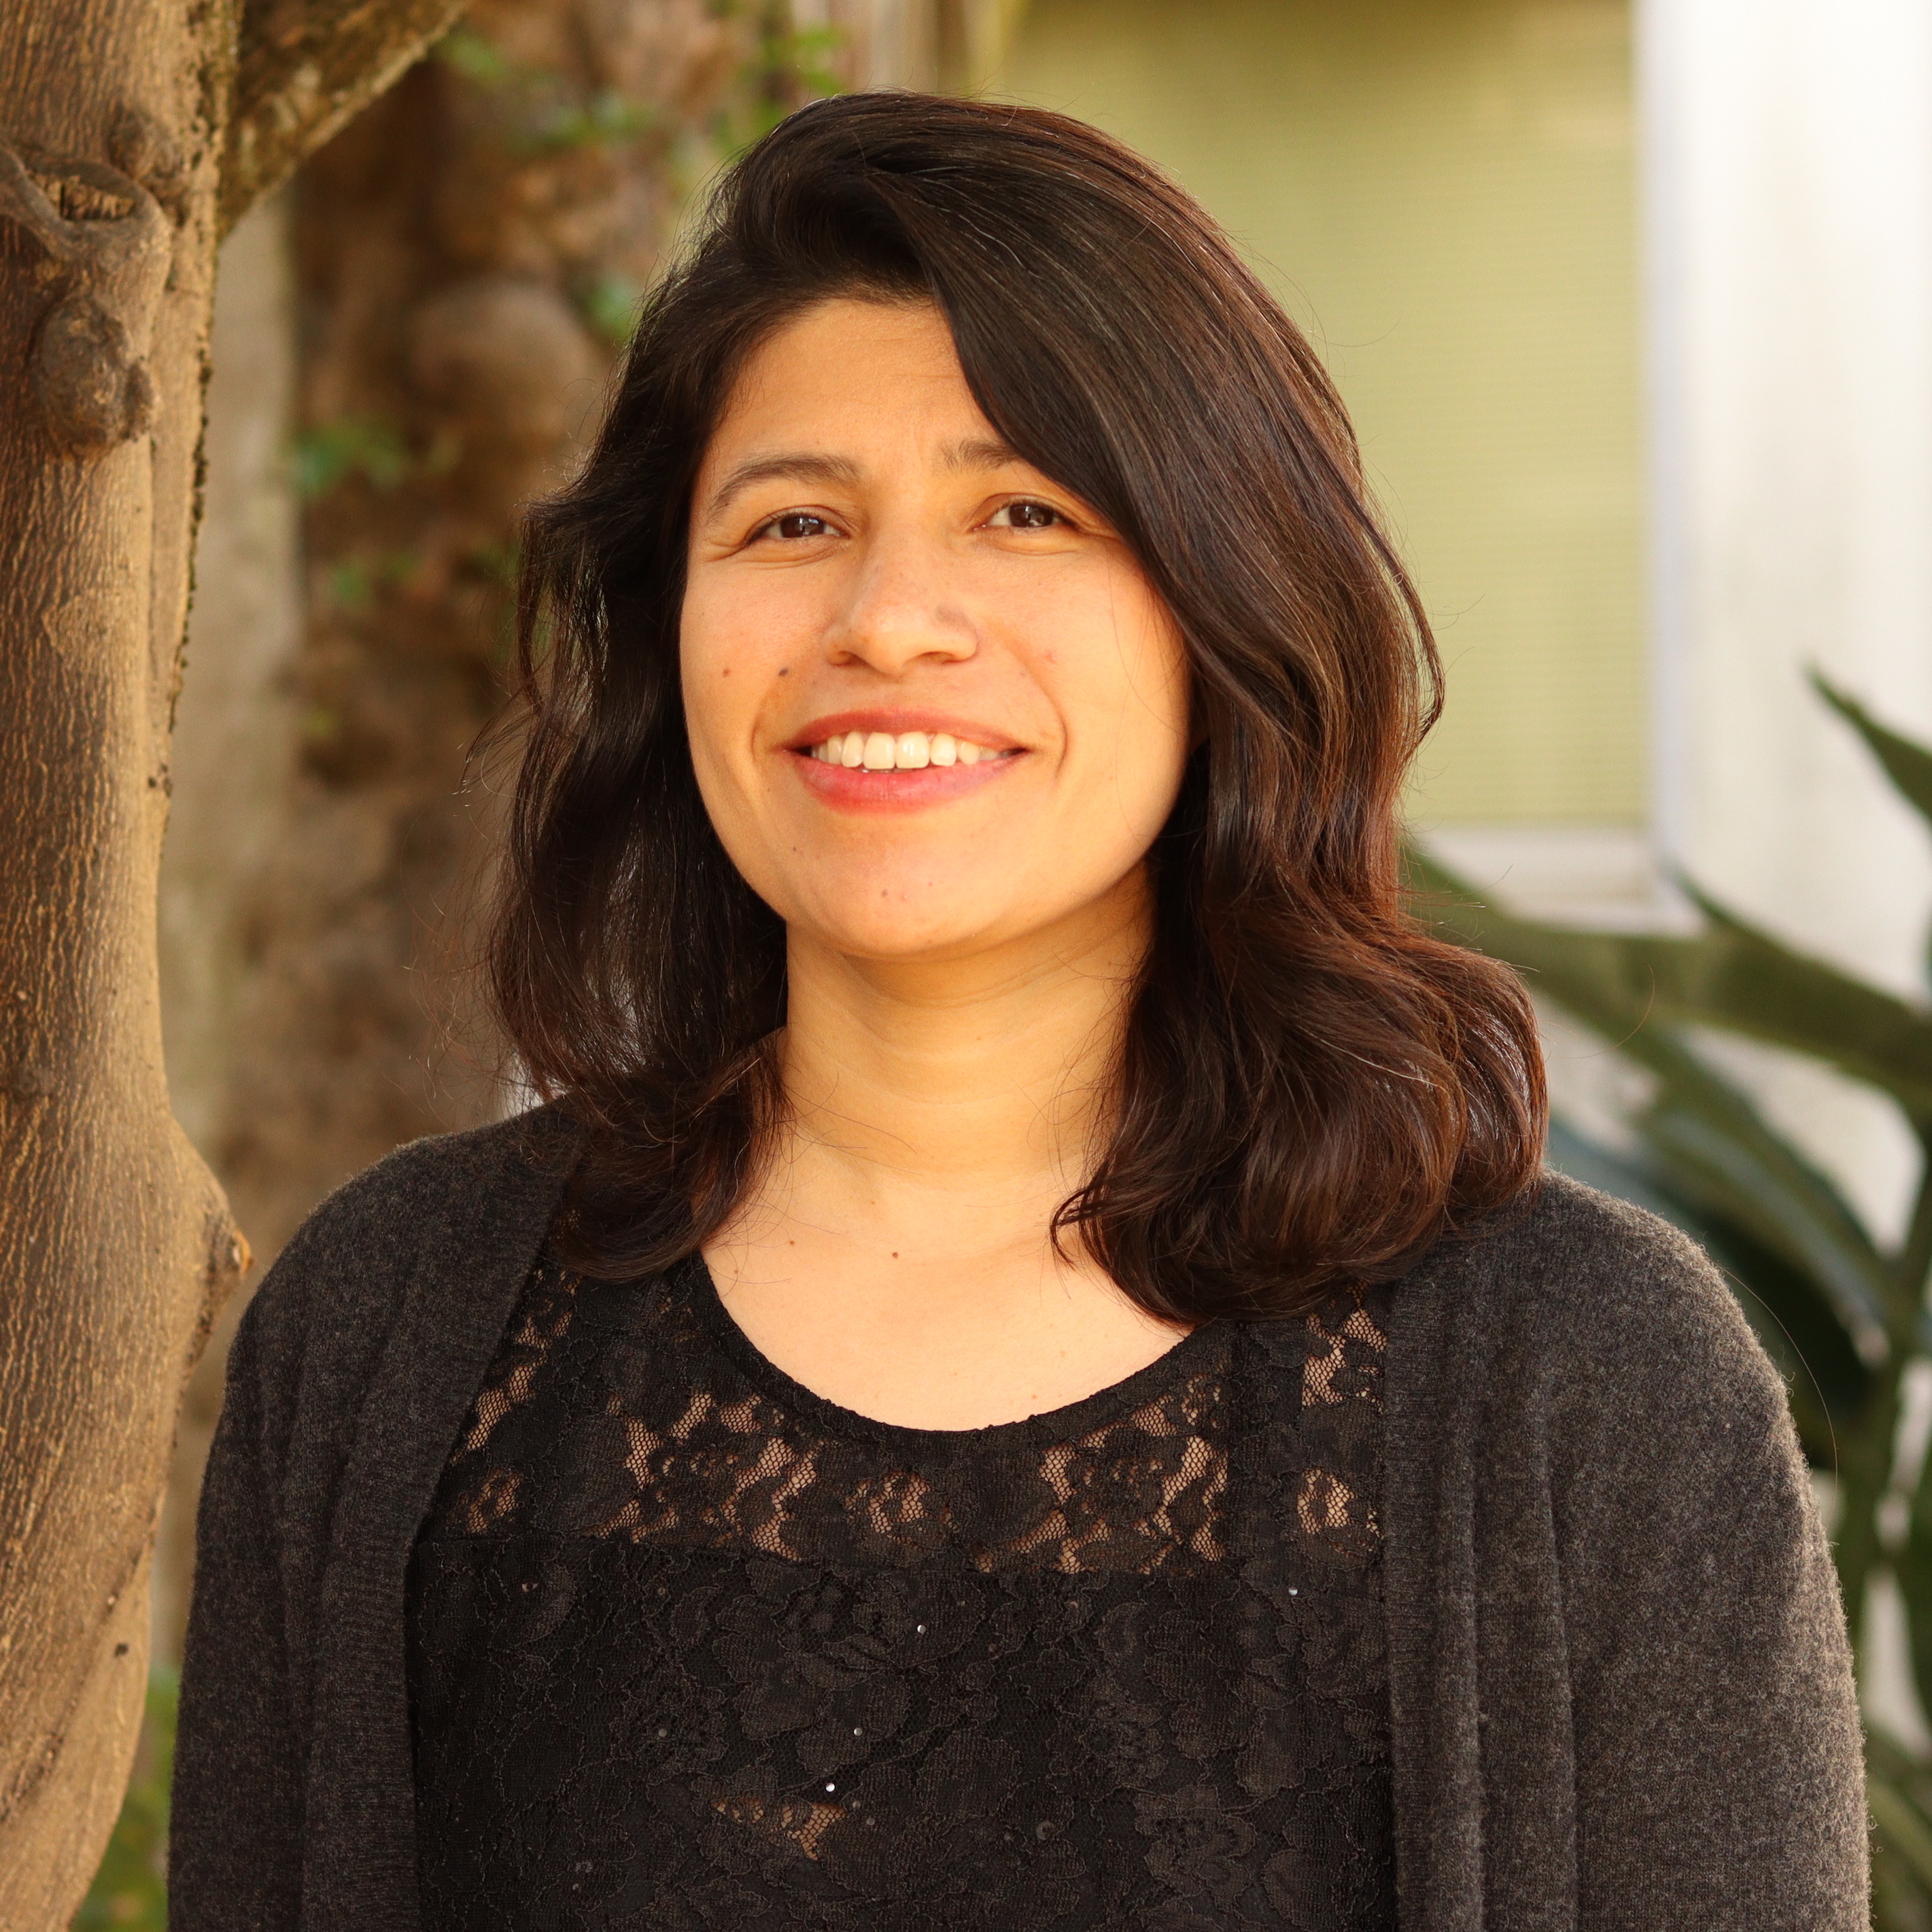
\includegraphics[width=0.25\textwidth]{photo.JPG}   \end{minipage} 
\end{tabular*}
%-----------------------------------------------------------

\vspace{0.2cm}

%-----------------------------------------------------------
\subsection*{Research Interests}

My research is focused on studying the self-assembly protein modules as the root cause of disease and to use this knowledge as a tool in synthetic biology to develop new diagnostics and therapeutic technologies. I use an interdisciplinary approach that includes cell-models, \textit{in vitro} and \textit{in vivo} biophysical assays, molecular simulations and protein engineering.

%-----------------------------------------------------------

\subsection*{Education, Research and Professional Experience}

\begin{itemize}

\item \textbf{2021 - present}. \textbf{Invited researcher}. Bionanotechnology and macromolecules Laboratory. Institute of Chemistry. National Autonomous University of Mexico   
  \textit{Subject}: New diagnostic tools based in CRISPR-Cas and isothermal amplification 

\item \textbf{2019 - 2021}. \textbf{Postdoctoral researcher}. Cell Structure and Dynamics Laboratory. Faculty of Science. University of Lisbon, Portugal.   % 01/07/2019 - present
  \textit{Subject}: Influence of phosphorylation on huntingtin aggregation in a human cell line.%: the role of phosphorylation on aggresome formation and intracellular phase transitions.
  
\item \textbf{2018 - 2019}. \textbf{Invited researcher}. Biomolecular Self-Organization Laboratory. Institute of Chemical and Biological Technology. NOVA University of Lisbon. Portugal. % 01/11/2018 - 20/06/2019
 \textit{Subject}: Molecular mechanism of ATP as an hydrotope in A$\beta$ aggregation.
 
\item \textbf{2018}. \textbf{Invited researcher}. Department of Biochemistry and Structural Biology. Institute of Cell Physiology. The National Autonomous University of Mexico. Mexico.  % {} 01/02/2018 – 01/11/2018
  \textit{Subject}: Proprotein convertases dynamics upon inhibition by serpins.
  
 \item \textbf{2012 - 2017}. \textbf{Project Manager}. Mexican Protein Society. \textbf{2017 - 2018}.  %{01/04/2017 - 01/11/2018/}\\  01/04/2017 - 01/11/2018
\item \textbf{Ph.D.} Biophysical Chemistry Laboratory, Faculty of Chemistry,  The National Autonomous University of Mexico, Mexico*.   % 20/01/2012 - 28/02/2017
  \textit{Subject}: Flexibility and aggregation of $(\beta\alpha)_8$ barrels.
  
\item \textbf{2012}. \textbf{Research visitor}. Soft Matter and Molecular Biophysics Group, Department of Applied Physics, Faculty of Physics, University of Santiago de Compostela, Spain.  % () 20/01/2012 – 31/07/2012 
  \textit{Subject}: Microsecond-long all-atom molecular dynamics simulations of $(\beta\alpha)_8$ barrels 
  
\item \textbf{2009 - 2011}. \textbf{M.Sc.}  Department of Biochemistry and Structural Biology, Institute of Cell Physiology, The National Autonomous University of Mexico. Mexico.   % 03/02/2009 - 25/11/2011
  \textit{Subject}: Design of $(\beta\alpha)_8$ barrels chimeraes
  
\item \textbf{2009 - 2010}. \textbf{Research visitor}. Department of Chemistry and Physics, Faculty of Science, University of Granada. Granada, Spain.   % () 01/09/2009 – 31/01/2010
  \textit{Subject}: Protein Kinetic stability using an automated DSC
  
\item \textbf{2003 - 2008}. \textbf{B.Sc.} Department of Macromolecules, Institute of Chemistry, The National Autonomous University of Mexico. Mexico.  %  // 30/07/2007 – 26/11/2008 18/08/2003 - 26/11/2008 
  \textit{Dissertation Subject}: High-quality protein crystals using internal electric fields and cyclic voltammetry

\end{itemize}
%-----------------------------------------------------------
%\newpage
\subsection*{Publications}
\vspace*{0.2cm}
\nocitearticles{*} 
\bibliographystylearticles{plainyearrev}
\bibliographyarticles{articles} 
\textbf{*} \textit{Co-corresponding author} \\ %\vspace*{0.2cm}
%\hspace*{0.4cm}\textit{\small{Note: IF according to JCR, Quartiles according to Scimago }}% and Citations according to Google Scholar
\nociteunderreview{*}
\bibliographystyleunderreview{plainyearrev}
\bibliographyunderreview{underreview}
\nocitebookchaps{*}
\bibliographystylebookchaps{plainyearrev}
\bibliographybookchaps{bookchap}
\nociteproceedings{*}
\bibliographystyleproceedings{plainyearrev}
\bibliographyproceedings{proceedings}
\nocitepreparation{*}
\bibliographystylepreparation{plainyearrev}
\bibliographypreparation{preparation}
%-----------------------------------------------------------
\subsection*{Awards, Fellowships and Honors}
\begin{itemize}
    \item 2021 \textbf{Diversity Award}
    granted by The Protein Society
    \item 2018-2021 \textbf{Fellowship} from the Mexican Federal Government for a postdoctoral stay awarded by the National Council of Sciences and Technology (CONACyT)
    \item 2017-2018 \textbf{Grant} from the Mexican Federal Government under the \textit{Thematic Networks Program} awarded by the National Council of Sciences and Technology (CONACyT)
    \item 2017 \textbf{Cum Laude} PhD dissertation: "Protein flexibility and kinetic stability: the Trypanosomatidae's Triosephosphate Isomerase case"
 \item 2016 \textbf{Grant} from the Mexican Federal Government under the \textit{Research Assistants Program} awarded by the National Investigators System (SNI)
\item 2012-2015 \textbf{Fellowship} from the Mexican Federal Government for PhD studies awarded by the National Council of Sciences and Technology (CONACyT)
 \item 2012 \textbf{Fellowship} from the Mexican Federal Government for a short research stay at the University of Santiago de Compostela, Spain
 \item 2012 \textbf{Travel Award} from the Biochemistry PhD Program at UNAM for a short research stay at the University of Santiago de Compostela, Spain 
 \item 2010-2012 \textbf{Fellowship} for MsC studies granted by the Mexican National Council of Sciences and Technology (CONACyT)
  \item 2009 \textbf{Fellowship} from the Mexican Federal Government for a short research stay at the University of Granada, Spain
  \item 2009 \textbf{Travel Award} from the Biochemistry PhD Program at UNAM for a short research stay at the University of Granada, Spain 
 \item 2008 \textbf{Cum Laude} Bachelor dissertation: "Growing protein crystal under electric fields"
 \item 2008 \textbf{Travel Award} to attend the 12th International Conference on the Crystallization of Biological Macromolecules awarded by the organizer committee. 
 \item 2007-2008 \textbf{Grant} under the \textit{Research Assistant Program} awarded by the National Investigators System (SNI) for undergraduate research stay at the Institute of Chemistry, UNAM
\end{itemize}
%-----------------------------------------------------------
\subsection*{Volunteering}
\begin{itemize}
\item 2020 \textbf{COVID Testing Centre} at the Faculty of Science of the University of Lisbon. %Interview for TecReview: shorturl.at/rAEW5

\end{itemize}
%-----------------------------------------------------------
\subsection*{Skills}
\normalsize{\textbf{Technical}}
\begin{itemize}
    \item Atomic Force Microscopy, Widefield and Confocal Fluorescence Microscopy, Dynamic Light Scattering, Circular Dichroism, Differential Scanning Calorimetry, Isothermal Scanning Calorimetry, PCR, Immunocytochemistry, WB.
\end{itemize}
\normalsize{\textbf{Bench}}
\begin{itemize}
    \item Mammalian Cell Culture, Live-Cell Imaging, Molecular Biology, Protein Engineering, Biochemical Assays, Flow Cytommetry
\end{itemize}
\normalsize{\textbf{Computer}}
\begin{itemize}
    \item Programming: Python, R, MATLAB
     \item Typography: \LaTeX, Markdown, LibreOffice/OpenOffice, Microsoft Office
    \item Other: ImageJ scripting, UNIX scripting, numpy, Gromacs, AMBER
\end{itemize}
%-----------------------------------------------------------

\subsection*{Teaching and Tutoring}
\begin{itemize}
\item \textbf{Tutoring} 2020 Bachelor and PhD students at the Faculty of Science, University of Lisbon, Portugal  
\item \textbf{Tutoring} 2019 PhD students at ITQB-NOVA, Oeiras, Portugal
\item \textbf{Tutoring} 2020 \textit{Daria Kovalchuk} (Bachelor student). Cell Structure and Dynamics Laboratory, Faculty of Science, University of Lisbon, Portugal  
\item \textbf{Tutoring} 2019 \textit{Fabiana Miraglia} (PhD student). Cell Structure and Dynamics Laboratory, Faculty of Science, University of Lisbon, Portugal 
\item \textbf{Tutoring} 2019 \textit{Silvia Galderisi} (PhD student). Biomolecular Self-Organization Laboratory, ITQB-NOVA, Oeiras, Portugal 
  \item \textbf{Invited lecturer} Nov 2018. Biochemistry Grad School. Class Title “Protein purification and characterization techniques”. Institute of Cell Physiology, The National Autonomous University of Mexico, Mexico City. \textit{Subject:} Protein Thermodynamics.
 \item \textbf{Lecturer} Ago 2013 - Nov 2018 Thermodynamics. Undergraduate course at Faculty of Chemistry. UNAM, Mexico City. %05/08/2013 – 01/11/2018
 \end{itemize}
%-----------------------------------------------------------
\subsection*{Communications}
\normalsize{\textbf{Oral communications and invited talks}}
\begin{enumerate}
\item Guilherme G. Moreira, \textbf{Andrea Quezada}, Federico Herrera, Claudio M. Gomes. The S100B chaperone precludes formation of Tau puncta and liquid-liquid phase separation. \emph{PhasAGE International Conference "Phase transitions in aging and age-related diseases". Online event.} \textbf{2021}.  
\item \textbf{Andrea Quezada}, Daria Kovalchuk, Federico Herrera. N-terminal phosphorylation of Hungtintin exon 1 shifts its liquid-liquid phase separation diagram and alters the kinetics of aggresome formation in mammalian cells \emph{XXI SPB Biochemistry Congress 2020. Online event.} \textbf{2020}.
\item \textbf{Andrea Quezada}. Invited talk: "Huntingtin aggregation in live cells: amyloidogenesis, phase separation and aggresomes"  3er Coloquio en Materiales de Interés Biotecnológico “Perspectivas en la Salud Humana” (CMIB-2020), \emph{Universidad de Sonora, Mexico.} \textbf{2020}.
 \item \textbf{Andrea Quezada}. Invited talk: ``How to modify the kinetic stability of proteins using molecular dynamics simulations?'' Instituto Potosino de Investigación Científica y Tecnológica A.C., \emph{San Luis Potosí, Mexico.} \textbf{2017}.
 \item \textbf{Andrea Quezada}, Jessica Diaz-Salazar, Nallely Cabrera, Ruy Perez-Montfort, Ángel Piñeiro and Miguel Costas. Interplay between Protein Thermal Flexibility and Kinetic Stability. \emph{6th Congress of the Mexican Protein Society, Durango, Mexico.} \textbf{2017}. % 6-10 nov
  \item \textbf{Andrea Quezada}, Nallely Cabrera, Ruy Perez-Montfort, Ángel Piñeiro and Miguel Costas. The structural basis of protein kinetic stability: the Trypanosomatidae's TIM case. \emph{4th Congress of the Mexican Protein Society, Guanajuato, Mexico.} \textbf{2013}.
\end{enumerate}
\normalsize{\textbf{Poster communications}}
\begin{enumerate}
\item Miguel Costas, \textbf{Andrea Quezada}, and Ángel Piñeiro. Interplay between protein kinetic stability and thermal flexibility. \emph{42nd FEBS Congress: from molecules to cells and back, Jerusalem, Israel.} \textbf{2017}  %. 10-14 September
\item Angel Piñeiro, Miguel Costas and \textbf{Andrea Quezada}.Key structural differences between TbTIM and TcTIM revealed by thermal unfolding molecular dynamics simulations. \emph{29th Annual Symposium of the Protein-Society, Barcelona, Spain.} \textbf{2015} %21-25 July
\item \textbf{Andrea Quezada}, Angel Piñeiro and Miguel Costas.Temperature-induced unfolding molecular dynamics simulations of the triosephosphase isomerase of \textit{Trypanosoma cruzi} and \textit{Trypanosoma brucei}. \emph{XXIX Congress of the Mexican Biochemistry Society, Oaxaca, Oaxaca.} \textbf{2012} % 11-17 noviembre
\item \textbf {Andrea Quezada} and Miguel Costas. Kinetic stability of TIM chimeric enzymes. \emph{3rd Congress of the Mexican Protein Society, Mexico City, Mexico.} \textbf{2011}.
\item \textbf{Andrea Quezada} and Miguel Costas. Kinetic stability of chimeric enzymes from the triosephosphase isomerase of \textit{Trypanosoma cruzi} and \textit{Trypanosoma brucei}. \emph{XXVIII Congress of the Mexican Biochemistry Society, Tuxtla Gutiérrez, Chiapas.} \textbf{2011}. % 7-12 noviembre 
\item \textbf{Andrea Quezada} and Abel Moreno. Effect of an electromagnetic field on the crystallization of ferritin. \emph{12th International Conference on the Crystallization of Biological Macromolecules, Cancún, México.} \textbf{2008}. %, 6 - 9 de mayo de 2008
\end{enumerate}

%-----------------------------------------------------------

\subsection*{Outreach activities}

\begin{itemize}
\item 2020 - Short communication "N-terminal phosphorylation of Huntingtin exon 1: liquid-liquid phase separation and aggresome formation in mammalian cells".  Ciências Research Day, Faculty of Science, University of Lisbon, Portugal.
\item 2019 - present \textbf{Científicæs Mexicanæs en el Extranjero}  \textit{Member \& Co-Founder}. Twitter: @MexiCiencia.  Website: https://mexiciencia.github.io

\item 2017-2018 Project Manager at the Mexican Protein Society \\ %{01/04/2017 - 01/11/2018/}\\
\begin{itemize}
\item [i.] 10 Schools on Protein Science in ten different states of Mexico, with 1,534 students and 43 national speakers. \\
\item [ii.] 6 Workshops on Protein Science in four different states of the country, with 292 attendees, 30 national speakers and nine international speakers.
\item [iii.] 2 Annual Meetings of the Mexican Protein Society with 82 attendees.
\item [iv.] 2 Meetings to promote links between Academy, Industry and Decision-makers with  82 attendees.
\end{itemize}
\end{itemize}

%-----------------------------------------------------------

\subsection*{Research grants}
%-----------------------------------------------------------
\subsection*{Memberships}
\begin{itemize}
\item The Protein Society (2021)
\item Mexican Bioinformatics Network (2021)
\item Portuguese Biochemistry Society (2020)
\item Mexican Protein Society (2018-present)
\item Mexican Biochemistry Society (2012-2016)
\end{itemize}
%-----------------------------------------------------------

\subsection*{Other Professional activities}
 %Reviewer for international journals, Meeting organizer, Scientific advisor
%-----------------------------------------------------------
\subsection*{Training and Courses}
\begin{itemize}
\item \textbf{Introduction to GitHub for R} (2021) Mexican Bioinformatics Network - 3.5 hrs
\item \textbf{Grant Writing Course} (2019) Instituto de Tecnologia Química e Biologica - 18 hrs
\item \textbf{Python Course} by Dr. Manuel Nuno Melo (2018) Instituto de Tecnologia Química e Biologica - 16 hrs
\item \textbf{Workshop on Single-molecule techniques} (2018) Institute of Biotechnology, Universidad Nacional Autonoma de Mexico, Cuernavaca, Morelos, Mexico - 30 hrs 
\item \textbf{Workshop on Nuclear Magnetic Resonance of Proteins} (2018) - Centro de investigación de estudios avanzados, Mexico City - 22 hrs
\item \textbf{Introduction to Scientific Advice for Policy Making} (2018) - Centro de investigación de estudios avanzados, Mexico City - 18 hrs
\item \textbf{Course in Molecular modelling and dynamics} by Dr. Marcelino Arciniega (2018) - Institute of Cell Physiology - Universidad Nacional Autonoma de Mexico - 48 hrs 
\item \textbf{Minicourse in Protein Physics} by Dr. Paolo Carloni (2017) - Cuernavaca, Mexico. - 20 hrs
\item \textbf{Workshop on X-ray Scattering in Biology and Material Science`} (2017) Institute of Chemistry, Universidad Nacional Autonoma de Mexico - 8 hrs
\item \textbf{Workshop on Enhanced Sampling Molecular Dynamics Simulations} (2017) Faculty of Chemistry, Universidad Nacional Autonoma de Mexico - 20 hrs
\item \textbf{Course in Intellectual property rights and Entrepeneurship in Biotechnology} (2017) Institute of Biotechnology, Universidad Nacional Autonoma de Mexico, Cuernavaca, Morelos, Mexico - 8 hrs 
\item \textbf{3rd USA-Mexico Workshop in Biological Chemistry: Protein Folding, Dynamics and Function} (2013) Guanajuato, Mexico - 20 hrs
\item \textbf{2nd USA-Mexico Workshop in Biological Chemistry: Protein Folding, Misfolding and Design} (2011) Universidad Nacional Autonoma de Mexico, Mexico. March 18-21
\item \textbf{Introduction to Molecular Dynamics Simulations Workshop} by Dr. Angel Pineiro (2011) - Faculty of Chemistry, Universidad Nacional Autonoma de Mexico - 16 hrs
\item \textbf{International School on Macromolecules Crystallization} (2008) Cancún, México - 16 hrs
\end{itemize}
%-----------------------------------------------------------
\subsection*{Languages}
\begin{itemize}
    \item Spanish - Native speaker
    \item English -
    Speaking: Advanced (C1); Reading: Advanced (C1); 
   Writing: Advanced (C1); Listening: Advanced (C1);
    Peer-review: Advanced (C1)
    \item Portuguese - 
    Speaking: Intermediate (B1); Reading: Upper Intermediate (B2);
    Writing: Elementary (A2); Listening: Intermediate (B1);
    Peer-review: Beginner (A1)

\end{itemize}   
\hspace{0.4cm}\textbf{*} According to Europass Standards \small{(http://europass.cedefop.europa.eu/LanguageSelfAssessmentGrid/en)}
%-----------------------------------------------------------
\subsection*{Referees}

\begin{multicols}{2}
\begin{itemize}

\item Professor Federico Herrera \\
Cell Structure and Dynamics Laboratory \\
Faculty of Sciences, University of Lisbon \\
Phone: (+351) 92 500 9786 \\
Email: fherrera@fc.ul.pt

 \item Professor Claudio M. Gomes \\
 Protein Misfolding and Amyloids in Biomedicine Laboratory \\
 Faculty of Sciences, University of Lisbon \\
 Phone: (+351) 21 750 0256  \\
 Email: cmgomes@fc.ul.pt 

\item Professor Marcelino Arciniega \\
Biochemistry and Structural Biology \\
Institute of Cell Physiology \\
National Autonomous University of Mexico \\
Phone: +52 55 56 22 57 00 \\
Email: marciniega@ifc.unam.mx

\item Professor Armando Hernandez \\
Chemistry of Biomacromolecules \\
Institute of Chemistry \\
National Autonomous University of Mexico \\
Phone: +52 55 56 22 45 48 \\
Email: armandohg@iquimica.unam.mx


\end{itemize}
\end{multicols}

%-----------------------------------------------------------
\end{document}
